\documentclass{article}

\usepackage[english]{babel}

% Set page size and margins
% Replace `letterpaper' with `a4paper' for UK/EU standard size
\usepackage[letterpaper,top=2cm,bottom=2cm,left=3cm,right=3cm,marginparwidth=1.75cm]{geometry}
\usepackage{graphicx}

\title{Research Automation White Paper}
\author{Shiro Takagi}

\begin{document}
\maketitle

\section{What is Research?}

\subsection{The Working Definition of Research}
Research is the act of generating new knowledge. In other words, it can be thought of as an endeavor to make the unknown known.

\subsection{The Patterns in Research}

It is believed that research began with individual and concrete tasks. Among them, common actions were patterned and crystallized as a scientific method. We currently recognize this abstract set of behaviors as research. For example, hypothetico-deductive method and hypothesis testing are abstracted scientific method.

Also, researchers use a research paper as a medium of knowledge transfer. Therefore, there are patterned activities related to a research paper. Examples of these include conducting surveys, gathering information from papers, and writing a thesis.

Note that these are necessary tasks just because we use a paper as a medium of knowledge transfer, but they may not necessarily be indispensable for generating new knowledge. There are other such tasks as well. For example, peer review and fund raising are essential to current research practices in society, but they may not necessarily be indispensable for knowledge production.

In this way, various tasks arise in conjunction with research. When considering the automation and optimization of research, it is desirable to consider streamlining all of these tasks. However, in this article, we focus on the process from determining a research topic to publishing a research paper. We will refer to this process simply as the \textit{research process} from here on.

\subsection{Research Process}

\subsubsection{Overview}

As mentioned earlier, research is an attempt to turn the unknown into the known. Therefore, the research process can be seen as a function that takes the unknown as input and outputs the known. However, in reality, a single research paper may not be enough to turn the unknown into the known. Therefore, in practice, the research process is considered to be a procedure that takes the unknown as input, and outputs a text that describes the procedures and their results, as well as their interpretation, in order to turn the unknown into the known.

First, let me structure the common research process. In particular, I will base the structuring of the research process on the method of empirical science, which many researches rely on as a foundation. However, I believe that this framework can be applied to other research activities, such as mathematics, as well. I will explain the reason for this later.

The research process, especially that of empirical science, is carried out through the following steps: topic decision, hypothesis generation, verification design, verification, and analysis of experimental results. The outputs of these steps are then written into a paper, which undergoes peer review and is eventually published.

Note that some commonly seen items, such as surveys, are not included here for a reason. First, as mentioned earlier, gathering information from papers is only a means of knowledge transfer through the use of a thesis. Second, information extraction from papers can be done at any stage of the research process. Thus, I believe that processing related to a paper, such as \textit{reading papers} and \textit{writing a paper}, needs to be considered separately from the aforementioned research process.

Taking all of this into account, the research process can be expressed as follows:

\begin{figure}[h]
    \centering
    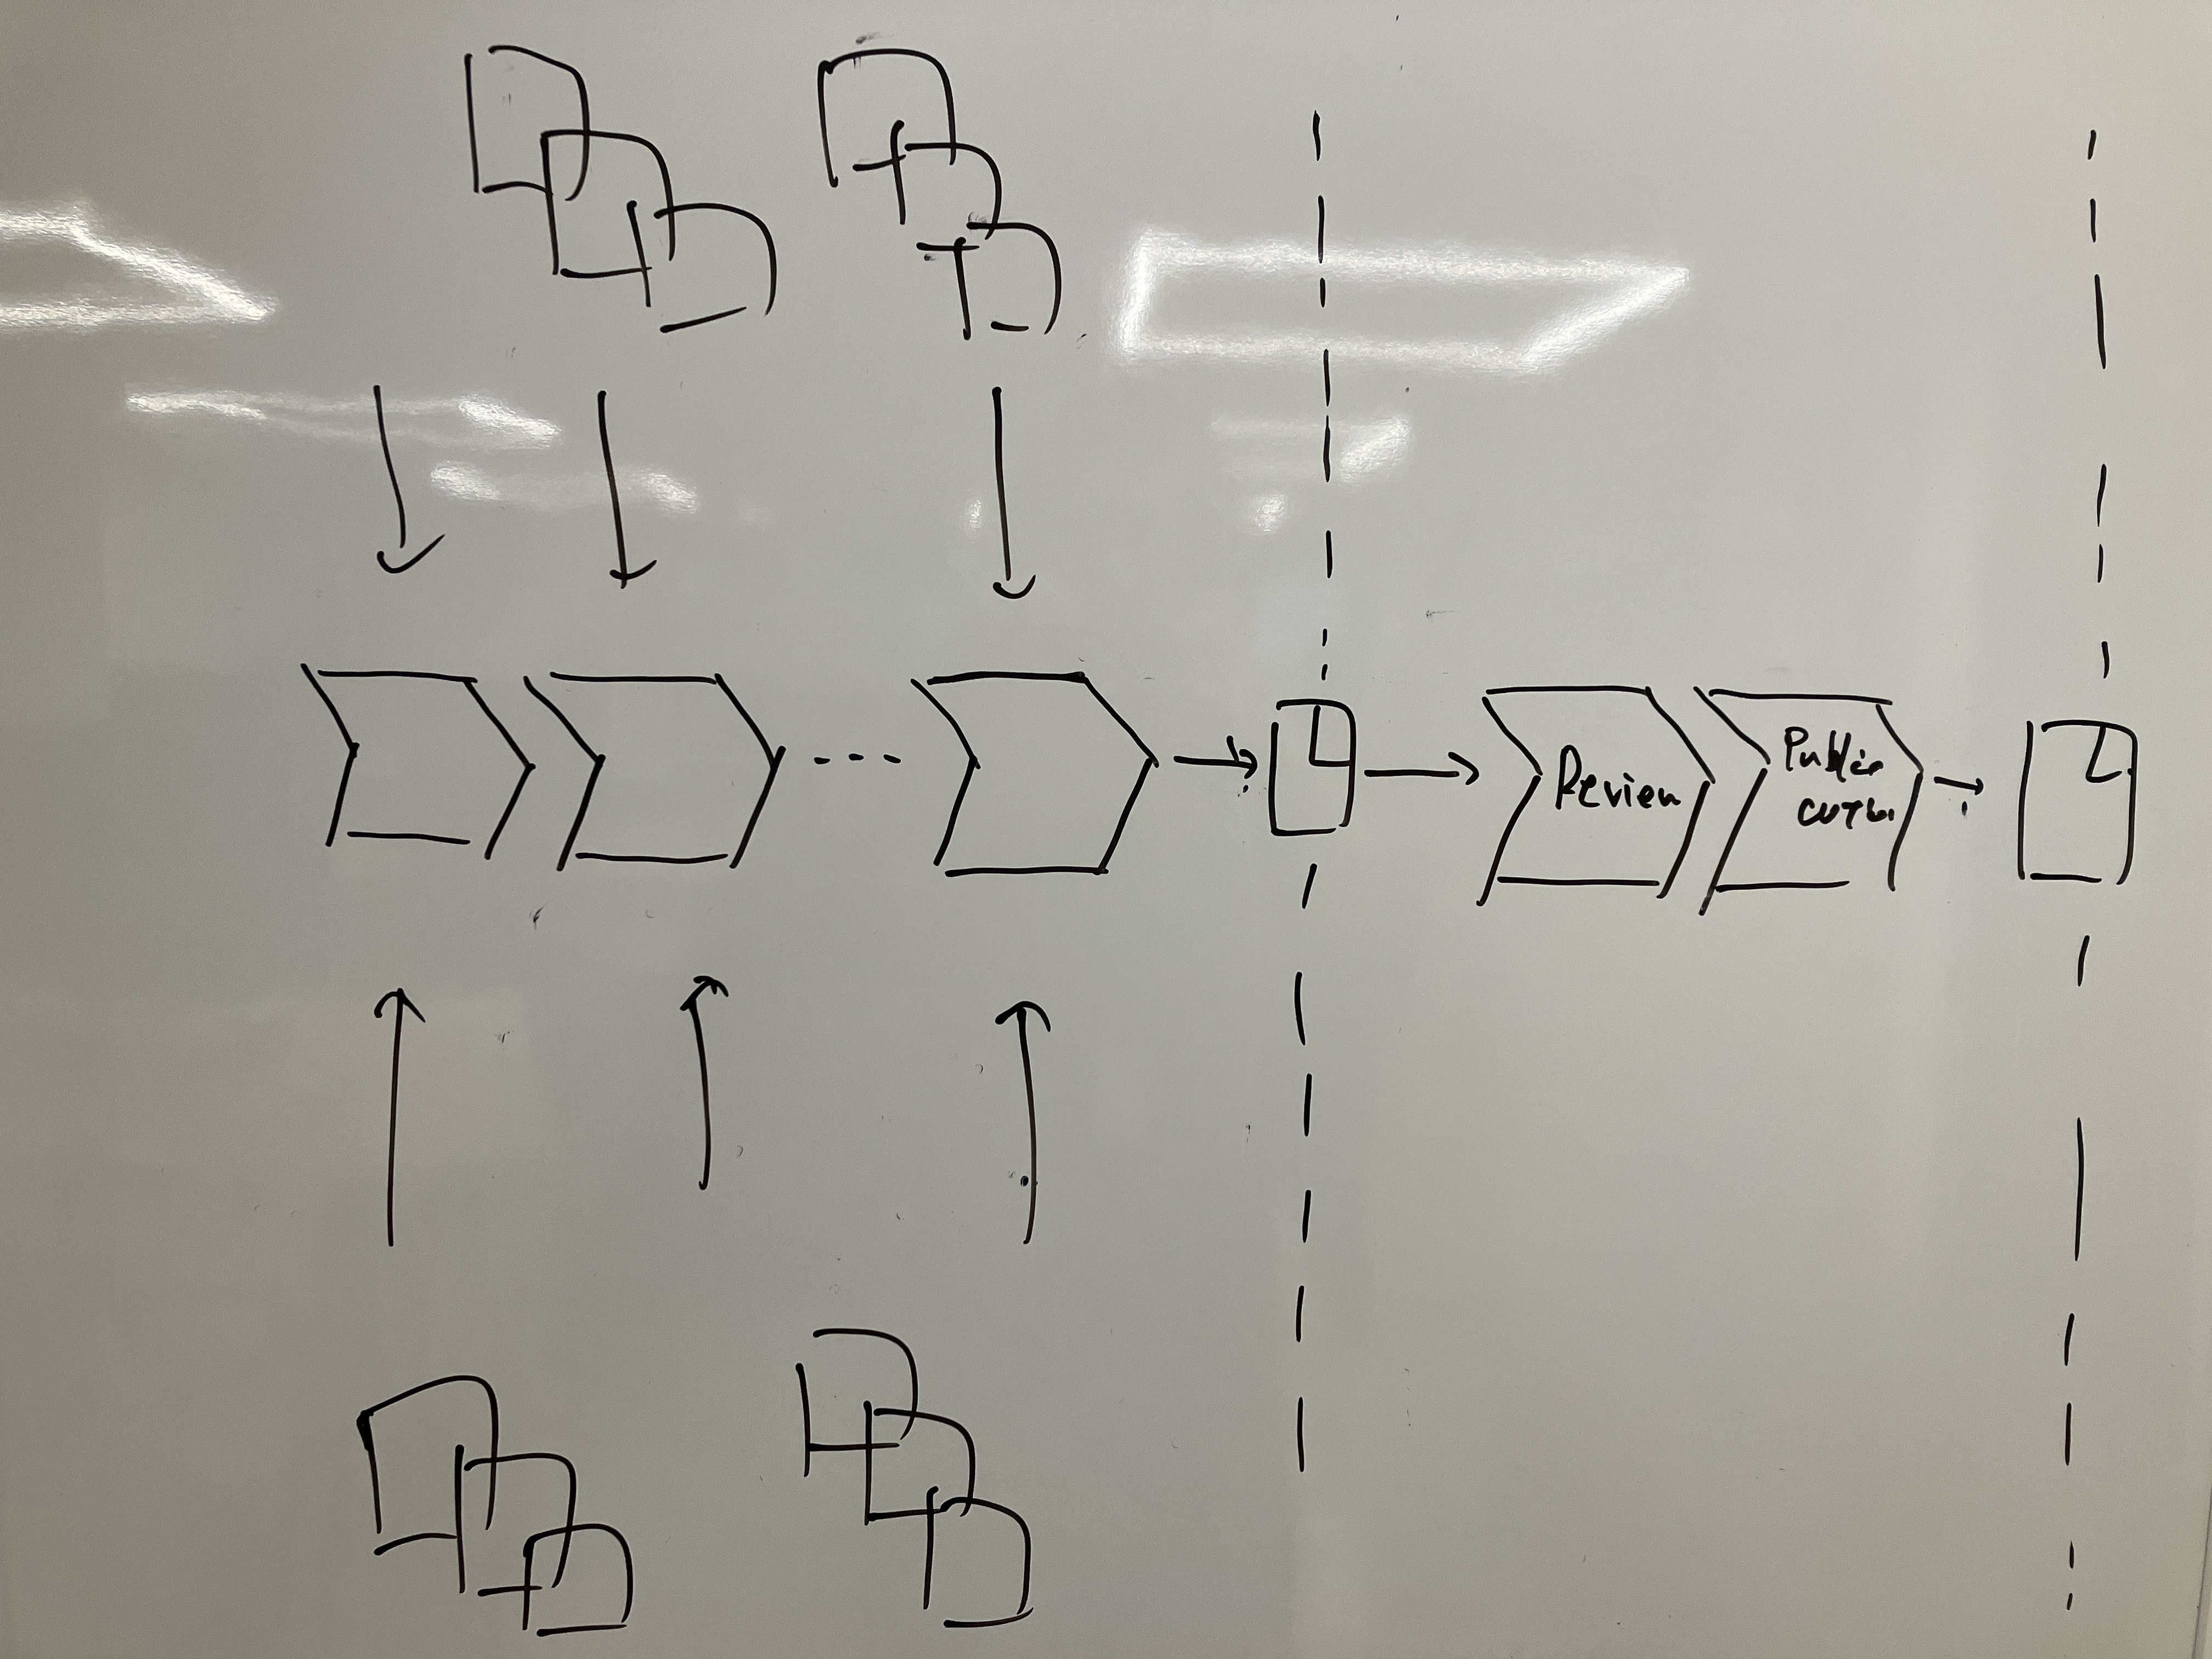
\includegraphics[width=\textwidth]{figs/researchprocess.jpg}
    \caption{Caption}
    \label{fig:research_process}
\end{figure}

This structuring is tentative and there may be a better way to structure the research process. However, I have created this structure for practical purposes in order to move the discussion forward. I will explain the reason for this division later. It is extremely important to consider research and, ultimately, the automation of research when thinking about better structuring. I hope the structure of this article be a starting point for conceiving a better structurization.

I will now proceed to a more detailed explanation of each step in the structured research process, followed by a separate discussion on reading and writing research papers.

\subsubsection{Topic Decision}
\subsubsection{Hypothesis Generation}
\subsubsection{Verification Design}
\subsubsection{Verification}
\subsubsection{Analysis}
\subsubsection{Paper Reading}
Survey (knowledge search + information acquisition and judgment from papers)

Knowledge search is necessary for information acquisition: knowledge search

It becomes necessary to judge not only single knowledge, but also to combine multiple knowledge: extraction of information from multiple papers and decision-making

Judgment of novelty and unknownness ← This is not involved in the entire process.
\subsubsection{Paper Writing}

Papers are assets, reports, and works.
"Importance" is explained in a way that conveys information value to readers and makes them look attractive.

It is assumed that humans will read it.

\section{Research Automation}

Automation of abstract processes

Automation of individual concrete processes

\section{Proposal}

Proposal for the progress of automation of individual tasks

Automation of tasks and fundamentally autonomous (end-to-end) research

Proposal for the progress towards the realization of intelligence that can autonomously conduct research.

\section{Conclusion}

\end{document}